\documentclass{article}
\usepackage{tikz}

\begin{document}

\begin{figure}[h]
    \centering
    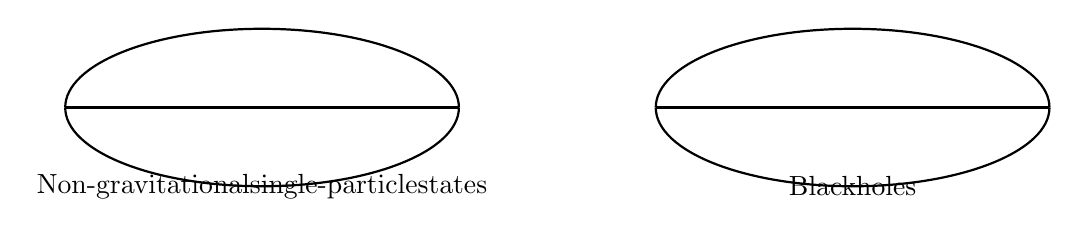
\begin{tikzpicture}[scale=0.5]
        % Non-gravitational single-particle states
        \draw[thick] (0,0) -- (10,0);
        \draw[thick] (0,0) arc (180:360:5 and 2);
        \draw[thick] (10,0) arc (0:180:5 and 2);
        
        % Black holes
        \draw[thick] (15,0) -- (25,0);
        \draw[thick] (15,0) arc (180:360:5 and 2);
        \draw[thick] (25,0) arc (0:180:5 and 2);
        
        % Labels
        \node at (5,-2) {Non-gravitational\\single-particle\\states};
        \node at (20,-2) {Black\\holes};
    \end{tikzpicture}
    \caption{Comparison of non-gravitational single-particle states and black holes.}
    \label{fig:comparison}
\end{figure}

\end{document}